  \documentclass{vldb}
\usepackage{graphicx}
\usepackage{balance}
\usepackage{fullpage}
\usepackage{graphicx,xspace,cite,verbatim,comment}
\usepackage{hyperref,array,color,balance,multirow}
\usepackage{caption,float,url,amsfonts}
\DeclareCaptionType{copyrightbox}
% \usepackage{rotating,amsmath,amsthm,amssymb}
\usepackage{color,cite,ifpdf,fancyvrb,array,listings}
% \usepackage{algorithm2e}
% \DeclarePairedDelimiter{\ceil}{\lceil}{\rceil}
% \DeclarePairedDelimiter{\floor}{\lfloor}{\rfloor}
% \DeclareMathOperator*{\argmin}{arg\,min}

\def\compactify{\itemsep=0pt \topsep=0pt \partopsep=0pt \parsep=0pt}
\let\latexusecounter=\usecounter
\newenvironment{CompactEnumerate}
 {\def\usecounter{\compactify\latexusecounter}
  \begin{enumerate}}
 {\end{enumerate}\let\usecounter=\latexusecounter}
\def\compactifytwo{\itemsep=-1pt \topsep=-1pt \partopsep=-2pt \parsep=-1pt \labelwidth=-2pt \leftmargin=-10pt}
\newenvironment{CompactItemize}
 {\def\usecounter{\latexusecounter}
  \begin{itemize}
  \compactifytwo
  }
 {\end{itemize}\let\usecounter=\latexusecounter}

\newtheorem{theorem}{Theorem}[section]
\newtheorem{proposition}{Proposition}[section]
\newtheorem{corollary}[theorem]{Corollary}
\newtheorem{lemma}[theorem]{Lemma}
\newcommand{\eat}[1]{}
\newcommand{\mat}[1]{{\mathbf{#1}}}
\renewcommand{\P}{\mathbb{P}}
\newcommand{\R}{\mathbb{R}}
\newcommand{\E}{\mathbb{E}}
\newcommand{\I}{\mathbb{I}}
\newcommand{\N}{\mathcal{N}}


\newenvironment{packeditems}{
\begin{itemize}
  \setlength{\itemsep}{1pt}
  \setlength{\parskip}{0pt}
  \setlength{\parsep}{0pt}
}{\end{itemize}}

\newenvironment{packedenums}{
\begin{enumerate}
  \setlength{\itemsep}{1pt}
  \setlength{\parskip}{0pt}
  \setlength{\parsep}{0pt}
}{\end{enumerate}}

\begin{document}

\title{Optimizing Stochastic Gradient Descent Over Normalized Data}


\maketitle

\begin{abstract}

\end{abstract}


\section{Introduction}

\paragraph*{Example}



\section{Preliminaries and Background}

\paragraph*{Generalized Linear Models (GLMs)}

\paragraph*{Stochastic Gradient Descent (SGD)}

\paragraph*{Problem Definition}



\section{Simple Approaches}

\subsection{SGD After a Join: Materialize}

\subsection{SGD Over a Join: Index-Stream}



\section{Optimizing SGD Over Joins}


\subsection{Order-Preserving Index-Stream under Low Memory}



\subsection{Order-Relaxed Approaches}

\subsubsection{Hash-Partitioned Index-Stream}

\paragraph*{Analysis of Relaxed Orderings}

\subsubsection{Simulation Study}

\subsubsection{Shuffling Only Once}


\subsection{Extensions}

\subsubsection{Multi-table Joins}
When the attribute tables cannot all entirely fit into the memory, multi-table joins introduce an optimization problem to HPIS.
\vspace{-1mm}
\paragraph*{Problem Statement}

Suppose there are $n$ attribute tables with size $r_i, i=1,2,...,n$. Total memory is $m$.
We assume $\sum_{i=1}^n r_i > m$. The amount of memory allocated to each table as $m_i$.
\begin{equation*}
\begin{aligned}
& \underset{m_i}{\text{min}}
& & \prod\limits_{i=1}^n \ceil{\frac{h.r_i}{m_i}} \\
& \text s.t.
& & \sum_{i=1}^n m_i = m, \\
&&& 1\le m_i\le m-n 
\end{aligned}
\end{equation*}

\paragraph*{Greedy Approach}
We relax the problem to:
\begin{equation*}
\begin{aligned}
& \underset{m_i}{\text{min}}
& & \prod\limits_{i=1}^n \frac{h.r_i}{m_i}
\end{aligned}
\end{equation*}
Since $h.r_i$ is fixed, this relaxed problem is equivalent to
\begin{equation*}
\begin{aligned}
& \underset{m_i}{\text{max}}
& & \prod\limits_{i=1}^n {m_i} \\
& \text s.t.
& & \sum_{i=1}^n m_i = m, \\
&&& 1\le m_i\le m-n 
\end{aligned}
\end{equation*}
For this problem, when $m_i = \bar{m}$, we have the optima.
Our greedy approach starts from here and make minimal 
adjustments to approach optima of the original problem. \\
For tables that are smaller than the initial mean, 
they are given memory no more than their size. 
The rest memory and the rest R tables become a subproblem 
same as the original problem. We recalculate the mean based 
on the rest memory and the rest R tables. Doing this recursively, 
we stop when the rest R tables are all larger than the current mean. \\
Let $P_i$ be the current number of partitions of $R_i$. 
For the rest of this approach, we are going to introduce 2 measures. \\
$cost_i=\ceil{\frac{r_i\mod m_i}{P_i-1}}$ \\
$surplus_i=\ceil{\frac{m_i-r_i\mod m_i}{P_i}}-1$ \\
$R_i$ needs $cost$ more pages to reduce its number of partitions.
And it can give at most $surplus$ more pages to not increase its number of partitions.

\begin{algorithm}[t]
Array $v \leftarrow 2$ attribute tables' info
$\bar{m} \leftarrow \frac{m}{n}$ 

\While{there is $v_i$ smaller than $\bar{m}$}{
Delete $v_i$ \\
$n \leftarrow n-1$ \\
$\bar{m} = \frac{m-v_i}{n}$
}
\While{$v$ is not empty and $\sum surplus > cost_{lowest}$}{
  Choose $v_i$ with the lowest cost. \\
  $v_{target}=v_i$. \\
  Erase $v_i$ from the array $v$. \\
  Sort $v$ on surplus. \\
  \For{i=1 to $v.size()$}{
    $cost_{target}-=min(cost_{target},  surplus_i)$ \\
    update $v_i$ \\
     \If {$cost_{target}==0$}{
        break;
     }
  }
}

\end{algorithm}

\paragraph*{Comparing performance of different partition algorithms}

\begin{figure}[h]
\centering
\includegraphics[width=3.0in]{HPIS_code/Synthetic/plot/random_data/Plot3}
\caption{Comparison of convergence speed with 2 R tables}
\end{figure}

\begin{figure}[h]
\centering
\includegraphics[width=3.0in]{HPIS_code/Synthetic/plot/random_data/Plot4}
\caption{Comparison of convergence speed with 4 R tables}
\end{figure}

\begin{figure}[h]
\centering
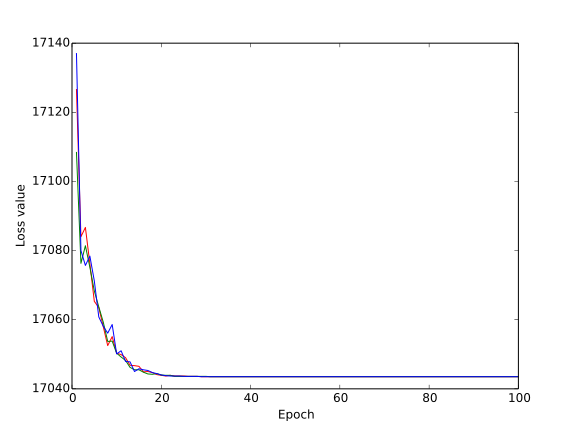
\includegraphics[width=3.0in]{HPIS_code/Synthetic/plot/random_data/Plot5}
\caption{Comparison of convergence speed with 6 R tables}
\end{figure}

The plots show the learning convergence speed of three partition methods: optimal solution which looks at all possible partitions, greedy solution mentioned above, and partitioning proportional to the size of each R table. The experiment is run on synthetic data with 2, 4, and 6 R tables. In cases we tested, all algorithms are able to converge quickly after a few epochs, and we also found that in most cases the difference in total number of chunks in R tables is not significant between the greedy search and optimal search.

\subsubsection{Shared-nothing Parallelism}


\subsection{Mini-Batch Gradient Descent}


\section{Experiments}

We implement our HPIS algorithm with user-defined functions in postgreSQL.
It is run on machines with 2 Intel E5-2630 processors and 128 GB of ECC RAM.
In our experiment we have two memory buffer settings on the database when comparing materialized learning scheme with HPIS: when memory is constrained and cannot hold the full R table, hence the HPIS algorithm will split S and R into multiple chunks. In the other setting we set memory buffer to be large enough to hold R, but not enough to include the S table, and in this case we are essentially comparing Materialize with IS. We also compare the performance when different shuffling schemes: when we shuffle the S table after each epoch, or only once at the beginning.The extension runs the SGD over 100 epochs, and performance is compared over various tuple ratios ($n_S$:$n_R$),feature ratios ($d_R$:$d_S$),and a factor of chunk sizes.

\begin{figure}[h]
\centering
\includegraphics[width=3.0in]{salways_small}
\caption{Performance comparison with small memory buffer, shuffling after each epoch}
\includegraphics[width=3.0in]{sonce_small}
\caption{Performance comparison with constrained memory buffer, shuffling only at the beginning}

\end{figure}

With small memory setting, we see that HPIS does not gain much in terms of increasing tuple ratio, but has a clear advantage as the feature ratio increases. As size of R grows, performance of HPIS wins by avoiding random I/O cost of matching hash entries in R using HPIS. We also see more benefit of HPIS in shuffle always scheme, as we save the random I/O cost of shuffling large table T.

\begin{figure}[h]
\centering
\includegraphics[width=3.0in]{salways_large}
\caption{Performance comparison with large memory buffer, shuffling after each epoch}
\includegraphics[width=3.0in]{sonce_large}
\caption{Performance comparison with large memory buffer, shuffling only at the beginning}
\end{figure}

\paragraph{Effect of data shuffling when data is skewed}

Here we consider two ways data is skewed. In one way, we get all the positive samples before we hit the first negative sample. In the other way, the two classes of sample appear in a round-robin fashion: we see a small group of positive data, then a group of negative data, and so on. In this experiment we study in both cases, how does the number of partition chunks affect the convergence speed. We present three of the plots in each case with 4, 8, and 12 partition chunks. We find that even with skewed data, the convergence speed of HPIS remains stable when number of partition chunks increases.

\begin{figure}[h]
\centering
\includegraphics[width=3.0in]{half_half}
\caption{Convergence speed with 4,8,12 partition chunks on data separated into positive and negative groups}
\end{figure}

\begin{figure}[h]
\centering
\includegraphics[width=3.0in]{skewed_chunk}
\caption{Convergence speed with 4,8,12 partition chunks on data in groups and round-robin fashion}
\end{figure}

\paragraph*{Real Datasets}

\paragraph*{Experimental Setup}

\subsection{High-level Performance and Quality}

\subsection{Performance Drill-Down}

\subsection{Evaluation of Extensions}



\section{Related Work}



\section{Conclusion and Future Work}



{
\scriptsize
\bibliographystyle{abbrv}
\bibliography{SGDOverJoins}
}

\end{document}